\documentclass{article}
\usepackage[backend=biber,natbib=true,style=alphabetic,maxbibnames=50]{biblatex}
\addbibresource{/home/nqbh/reference/bib.bib}
\usepackage[utf8]{vietnam}
\usepackage{tocloft}
\renewcommand{\cftsecleader}{\cftdotfill{\cftdotsep}}
\usepackage[colorlinks=true,linkcolor=blue,urlcolor=red,citecolor=magenta]{hyperref}
\usepackage{amsmath,amssymb,amsthm,float,graphicx,mathtools,tikz}
\usetikzlibrary{angles,calc,intersections,matrix,patterns,quotes,shadings}
\allowdisplaybreaks
\newtheorem{assumption}{Assumption}
\newtheorem{baitoan}{Bài toán}
\newtheorem{cauhoi}{Câu hỏi}
\newtheorem{conjecture}{Conjecture}
\newtheorem{corollary}{Corollary}
\newtheorem{dangtoan}{Dạng toán}
\newtheorem{definition}{Definition}
\newtheorem{dinhly}{Định lý}
\newtheorem{dinhnghia}{Định nghĩa}
\newtheorem{example}{Example}
\newtheorem{ghichu}{Ghi chú}
\newtheorem{hequa}{Hệ quả}
\newtheorem{hypothesis}{Hypothesis}
\newtheorem{lemma}{Lemma}
\newtheorem{luuy}{Lưu ý}
\newtheorem{nhanxet}{Nhận xét}
\newtheorem{notation}{Notation}
\newtheorem{note}{Note}
\newtheorem{principle}{Principle}
\newtheorem{problem}{Problem}
\newtheorem{proposition}{Proposition}
\newtheorem{question}{Question}
\newtheorem{remark}{Remark}
\newtheorem{theorem}{Theorem}
\newtheorem{vidu}{Ví dụ}
\usepackage[left=1cm,right=1cm,top=5mm,bottom=5mm,footskip=4mm]{geometry}
\def\labelitemii{$\circ$}
\DeclareRobustCommand{\divby}{%
	\mathrel{\vbox{\baselineskip.65ex\lineskiplimit0pt\hbox{.}\hbox{.}\hbox{.}}}%
}

\title{Problem {\it\&} Solution: Trigonometry In Triangles\\Bài Tập \& Lời Giải: Hệ Thức Lượng Trong Tam Giác}
\author{Nguyễn Quản Bá Hồng\footnote{Independent Researcher, Ben Tre City, Vietnam\\e-mail: \texttt{nguyenquanbahong@gmail.com}; website: \url{https://nqbh.github.io}.}}
\date{\today}

\begin{document}
\maketitle
\begin{abstract}
	Last updated version: \href{https://github.com/NQBH/elementary_STEM_beyond/blob/main/elementary_mathematics/grade_9/trigonometry/problem/NQBH_trigonometry_problem.pdf}{GitHub{\tt/}NQBH{\tt/}elementary STEM \& beyond{\tt/}elementary mathematics{\tt/}grade 9{\tt/}trigonometry{\tt/}problem: set $\mathbb{Q}$ of trigonometrys [pdf]}.\footnote{\textsc{url}: \url{https://github.com/NQBH/elementary_STEM_beyond/blob/main/elementary_mathematics/grade_9/trigonometry/problem/NQBH_trigonometry_problem.pdf}.} [\href{https://github.com/NQBH/elementary_STEM_beyond/blob/main/elementary_mathematics/grade_9/trigonometry/problem/NQBH_trigonometry_problem.tex}{\TeX}]\footnote{\textsc{url}: \url{https://github.com/NQBH/elementary_STEM_beyond/blob/main/elementary_mathematics/grade_9/rational/problem/NQBH_trigonometry_problem.tex}.}. 
\end{abstract}
\tableofcontents

%------------------------------------------------------------------------------%

\section{1 Số Hệ Thức Lượng về Cạnh \& Đường Cao Trong Tam Giác Vuông}
\textbf{\textsf{Ký hiệu.}} $\Delta ABC$ vuông tại $A$: $a\coloneqq BC$, $b\coloneqq CA$, $c\coloneqq AB$, $b'\coloneqq CH$, $c'\coloneqq BH$, $h\coloneqq AH$.\\\textbf{\textsf{Tính chất.}} \fbox{1} $b^2 = ab'$, $c^2 = ac'$. \fbox{2} \textit{Định lý Pythagore thuận \& đảo}: $\Delta ABC$ vuông tại $A\Leftrightarrow a^2 = b^2 + c^2$. \fbox{3} $h^2 = b'c'$. \fbox{4} $ah = bc = 2S_{ABC}$. \fbox{5} $\dfrac{1}{h^2} = \dfrac{1}{b^2} + \dfrac{1}{c^2}$.

\begin{baitoan}[\cite{Binh_Toan_9_tap_1}, Ví dụ 1, p. 84]
	Tính diện tích hình thang ABCD có đường cao bằng {\rm12 cm}, 2 đường chéo AC, BD vuông góc với nhau, $BD = 15$ {\rm cm}.
\end{baitoan}

\begin{proof}[Giải]
	Kẻ $BE\parallel AC$, $E\in CD$. Gọi $BH$ là đường cao của hình thang. $BE\parallel AC$ \& $AC\bot BD\Rightarrow BE\bot BD$. Áp dụng định lý Pythagore cho $\Delta BDH$ vuông tại $H$: $HD = \sqrt{BD^2 - BH^2} = \sqrt{15^2 - 12^2} = \sqrt{225 - 144} = \sqrt{81} = 9$ cm. Áp dụng hệ thức lượng $b^2 = ab'$ vào $\Delta BDE$ vuông tại $B$: $DE = \dfrac{BD^2}{DH} = \dfrac{15^2}{9} = \dfrac{225}{9} = 25$ cm. $AB\parallel CE$ \& $AC\parallel BE\Rightarrow ABCE$ là hình bình hành $\Rightarrow AB = CE\Rightarrow AB + CD = CE + CD = DE = 25$ cm $\Rightarrow S_{ABCD} = \frac{1}{2}(AB + CD)\cdot BH = \frac{1}{2}\cdot25\cdot12 = 150\ {\rm cm}^2$.
\end{proof}

\begin{baitoan}[\cite{Binh_Toan_9_tap_1}, Ví dụ 2, p. 85]
	Hình thang cân ABCD có đáy lớn $CD = 10$ {\rm cm}, đáy nhỏ bằng đường cao, đường chéo vuông góc với cạnh bên. Tính đường cao của hình thang.
\end{baitoan}

\begin{proof}[Giải]
	Gọi $AH,BK$ là 2 đường cao của hình thang $ABCD$. Đặt $x\coloneqq AB = AH = BK$. Tứ giác $ABKH$ có $AB\parallel HK$, $AH\parallel BK$ (vì $AH\bot CD$ \& $BK\bot CD$) nên $ABKH$ là hình bình hành, mà $\widehat{H} = \widehat{K} = 90^\circ$ nên $ABKH$ là hình chữ nhật, kết hợp với $AB = AH$, suy ra $ABKH$ là hình vuông, nên $HK = AB = x$ (1). $ABCD$ là hình thang cân $\Rightarrow AD = BC$ \& $\widehat{C} = \widehat{D}$, suy ra $\Delta AHD = \Delta BKC$ (2 tam giác vuông lần lượt tại $H,K$, trường hợp cạnh huyền--góc nhọn\footnote{Hoặc có thể lý luận: $\Delta AHD = \Delta BKC$ (cạnh huyền--cạnh góc vuông) vì 2 tam giác vuông này có $AD = BC$ (2 cạnh bên của hình thang cân $ABCD$) \& $AH = BK$ (cùng bằng chiều cao của hình thang $ABCD$).}) $\Rightarrow DH = CK$ (2). Từ (1) \& (2), suy ra: $DH = CK = \dfrac{CD - HK}{2} = \dfrac{10 - x}{2}\Rightarrow CH = CK + HK = \dfrac{10 - x}{2} + x = \dfrac{10 + x}{2}$. Áp dụng hệ thức lượng $h^2 = b'c'$ cho $\Delta ACD$ vuông tại $A$ (đường chéo $AC\bot AD$: giả thiết): $AH^2 = DH\cdot CH\Leftrightarrow x^2 = \dfrac{10 + x}{2}\cdot\dfrac{10 - x}{2} = \dfrac{100 - x^2}{4}\Leftrightarrow4x^2 = 100 - x^2\Leftrightarrow5x^2 = 100\Leftrightarrow x = \sqrt{\dfrac{100}{5}} = \sqrt{20} = 2\sqrt{5}$ cm. Vậu đường cao của hình thang $ABCD$ bằng $2\sqrt{5}$ cm.
\end{proof}

\begin{baitoan}[\cite{Binh_Toan_9_tap_1}, Ví dụ 3, p. 85]
	Tính diện tích 1 tam giác vuông có chu vi {\rm72 cm}, hiệu giữa đường trung tuyến \& đường cao ứng với cạnh huyền bằng {\rm7 cm}.
\end{baitoan}

\begin{proof}[Giải]
	Xét $\Delta ABC$, $AB < AC$, $M$ là trung điểm $BC$, $AH\bot BC$, $H\in BC$, như hình:
	\begin{center}
		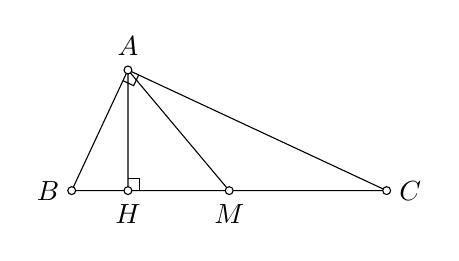
\begin{tikzpicture}
			\def\r{2}
			\path
			(130:\r) coordinate (A)
			(180:\r) coordinate (B)
			(0:\r) coordinate (C)
			($(B)!(A)!(C)$) coordinate (H)
			($(B)!.5!(C)$) coordinate (M)
			;
			\draw
			(A)--(B)--(C)--cycle (A)--(H) (A)--(M)
			pic[draw, angle radius=1.5mm]{right angle=B--A--C}
			pic[draw, angle radius=1.5mm]{right angle=A--H--C}
			;
			\foreach \x/\g in {A/90,B/180,C/0,H/-90,M/-90} \draw[fill=white] (\x) circle (.05) + (\g:.3) node{$\x$};
		\end{tikzpicture}
	\end{center}
	Đặt $x\coloneqq AM$, $BC = 2AM = 2x$, $AH = AM - 7 = x - 7$. Áp dụng định lý Pythagore \& hệ thức lượng $bc = ah$ cho $\Delta ABC$ vuông tại $A$: $b^2 + c^2 = a^2 = (2x)^2 = 4x^2$, $bc = ah = 2x(x - 7)$. Giải hệ phương trình:\footnote{Xem cách giải của dạng tổng quát của hệ phương trình này ở bài viết sau của tác giả: \textit{Problem \& Solution: System of Equations of 2 Variables -- Bài Tập \& Lời Giải: Hệ Phương Trình 2 Biến}: \textsc{url}: \url{https://github.com/NQBH/elementary_STEM_beyond/blob/main/elementary_mathematics/miscellaneous/system_of_equations_2_variables/problem/NQBH_system_of_equations_2_variables_problem.pdf}.}
	\begin{equation*}
		\left\{\begin{split}
			b^2 + c^2 &= 4x^2,\\
			bc &= 2x(x - 7).
		\end{split}\right.
	\end{equation*}
	Có $a + b + c = 72\Leftrightarrow b + c = 72 - a = 72 - 2x$. Từ hệ phương trình vừa thu được: $(b + c)^2 = b^2 + c^2 + 2bc = 4x^2 + 4x(x - 7) = 8x^2 - 28x\Leftrightarrow(72 - 2x)^2 = 8x^2 - 28x\Leftrightarrow72^2 - 2\cdot72\cdot2x + 4x^2 = 8x^2 - 28x\Leftrightarrow4x^2 + 260x - 72^2 = 0\Leftrightarrow x^2 + 65x - 1296 = 0\Leftrightarrow(x - 16)(x + 81) = 0\Leftrightarrow x = 16\lor x = -81$ (loại vì $x > 0$) $\Rightarrow x = 16\Rightarrow S_{ABC} = \frac{1}{2}bc = x(x - 7) = 16(16 - 7) = 144\ {\rm cm}^2$.
\end{proof}

\begin{baitoan}[\cite{Binh_Toan_9_tap_1}, 1., p. 86]
	Chứng minh định lý Pythagore bằng cách đặt 2 tam giác vuông bằng nhau $\Delta ABC = \Delta DCE$:
	\begin{center}
		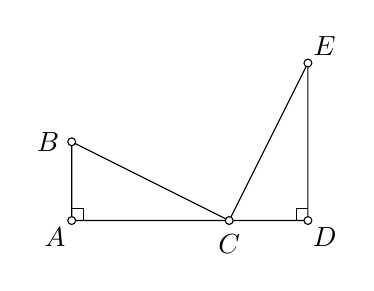
\begin{tikzpicture}
			\path
			(0,0) coordinate (A)
			(0,1) coordinate (B)
			(2,0) coordinate (C)
			(3,0) coordinate (D)
			(3,2) coordinate (E)
			;
			\draw
			(A)--(B)--(C)--cycle (C)--(D)--(E)--cycle
			pic[draw, angle radius=1.5mm]{right angle=B--A--C}
			pic[draw, angle radius=1.5mm]{right angle=C--D--E}
			;
			\foreach \x/\g in {A/-135,B/180,C/-90,D/-45,E/45} \draw[fill=white] (\x) circle (.05) + (\g:.3) node{$\x$};
		\end{tikzpicture}
	\end{center}
\end{baitoan}

\begin{baitoan}[\cite{Binh_Toan_9_tap_1}, 2., p. 86]
	Cho $\Delta ABC$ cân có $AB = AC = 9$ {\rm cm}, $BC = 12$ {\rm cm}, đường cao $AH$, I là hình chiếu của H trên AC. (a) Tính độ dài CI. (b) Kẻ đường cao BK của $\Delta ABC$. Chứng minh điểm K nằm giữa 2 điểm A, C.
\end{baitoan}

\begin{baitoan}[\cite{Binh_Toan_9_tap_1}, 3., p. 86]
	Cho $\Delta ABC$ có $\widehat{A} = 120^\circ$, $BC = a$, $AC = b$, $AB = c$. Chứng minh $a^2 = b^2 + c^2 + bc$.
\end{baitoan}

\begin{baitoan}[\cite{Binh_Toan_9_tap_1}, 4., p. 86]
	Tính cạnh đáy BC của $\Delta ABC$ cân biết đường cao ứng với cạnh đáy bằng {\rm15.6 cm} \& đường cao ứng với cạnh bên bằng {\rm12 cm}.
\end{baitoan}

\begin{baitoan}[\cite{Binh_Toan_9_tap_1}, 5., p. 86]
	Cho $\Delta ABC$ vuông tại A, đường phân giác AD, đường cao AH. Biết $BD = 7.5$ {\rm cm}, $CD = 10$ {\rm cm}. Tính AH, BH, DH.
\end{baitoan}

\begin{baitoan}[\cite{Binh_Toan_9_tap_1}, 6., p. 86]
	Cho $\Delta ABC$ vuông tại A, đường cao AH, $AB = 20$ {\rm cm}, $CH = 9$ {\rm cm}. Tính độ dài AH.
\end{baitoan}

\begin{baitoan}[\cite{Binh_Toan_9_tap_1}, 7., p. 86]
	Cho $\Delta ABC$ vuông tại A, đường cao AH. Tia phân giác của $\widehat{HAC}$ cắt HC ở D. Gọi K là hình chiếu của D trên AC. Biết $BC = 25$ {\rm cm}, $DK = 6$ {\rm cm}. Tính AB.
\end{baitoan}

\begin{baitoan}[\cite{Binh_Toan_9_tap_1}, 8., p. 86]
	Cho $\Delta ABC$ có $AB = 6$ {\rm cm}, $AC = 8$ {\rm cm}, 2 đường trung tuyến BD, CE vuông góc với nhau. Tính BC.
\end{baitoan}

\begin{baitoan}[\cite{Binh_Toan_9_tap_1}, 9., p. 86]
	Cho $\Delta ABC$ có $\widehat{B} = 60^\circ$, $BC = 8$ {\rm cm}, $AB + AC = 12$ {\rm cm}. Tính AB, AC.
\end{baitoan}

\begin{baitoan}[\cite{Binh_Toan_9_tap_1}, 10., p. 86]
	Trong 1 tam giác vuông, đường cao ứng với cạnh huyền chia tam giác thành 2 phần có diện tích bằng $\rm54\ cm^2$ \& $\rm96\ cm^2$. Tính độ dài cạnh huyền.
\end{baitoan}

\begin{baitoan}[\cite{Binh_Toan_9_tap_1}, 11., p. 86]
	Cho $\Delta ABC$ vuông cân tại A, đường trung tuyến BM. Gọi D là hình chiếu của C trên BM, H là hình chiếu của D trên AC. Chứng minh $AH = 3DH$.
\end{baitoan}

\begin{baitoan}[\cite{Binh_Toan_9_tap_1}, 12., pp. 86--87]
	(a) 1 tam giác vuông có tỷ số các cạnh góc vuông bằng $k$. Tính tỷ số các hình chiếu của 2 cạnh góc vuông trên cạnh huyền. (b) Tính độ dài hình chiếu của các cạnh góc vuông trên cạnh huyền của 1 tam giác vuông, biết tỷ số 2 cạnh góc vuông bằng $5:4$ \& cạnh huyền dài {\rm82 cm}.
\end{baitoan}

\begin{baitoan}[\cite{Binh_Toan_9_tap_1}, 13., p. 87]
	Trong 1 tam giác vuông, đường phân giác của góc vuông chia cạnh huyền thành 2 đoạn thẳng tỷ lệ với $1:3$. Đường cao ứng với cạnh huyền chia cạnh đó theo tỷ số nào?
\end{baitoan}

\begin{baitoan}[\cite{Binh_Toan_9_tap_1}, 14., p. 87]
	Cho $\Delta ABC$ có độ dài 3 cạnh AB, BC, CA là 3 số tự nhiên liên tiếp tăng dần. Kẻ đường cao AH, đường trung tuyến AM. Chứng minh $HM = 2$.
\end{baitoan}

\begin{baitoan}[\cite{Binh_Toan_9_tap_1}, 15., p. 87]
	1 hình thang cân có đường chéo vuông góc với cạnh bên. Tính chu vi \& diện tích hình thang biết đáy nhỏ dài {\rm14 cm}, đáy lớn dài {\rm50 cm}.
\end{baitoan}

\begin{baitoan}[\cite{Binh_Toan_9_tap_1}, 16., p. 87]
	1 hình thoi có diện tích bằng $\frac{1}{2}$ diện tích hình vuông có cạnh bằng cạnh của hình thoi. Tính tỷ số của đường chéo dài \& đường chéo ngắn của hình thoi.
\end{baitoan}

\begin{baitoan}[\cite{Binh_Toan_9_tap_1}, 17., p. 87]
	Qua đỉnh A của hình vuông ABCD cạnh $a$, vẽ 1 đường thẳng cắt cạnh BC ở M \& cắt đường thẳng CD ở I. Chứng minh $\dfrac{1}{AM^2} + \dfrac{1}{AI^2} = \dfrac{1}{a^2}$.
\end{baitoan}

\begin{baitoan}[\cite{Binh_Toan_9_tap_1}, 18., p. 87]
	Cho hình vuông ABCD có cạnh {\rm1 dm}. Tính cạnh của $\Delta AEF$ đều có E thuộc cạnh CD \& F thuộc cạnh BC.
\end{baitoan}

\begin{baitoan}[\cite{Binh_Toan_9_tap_1}, 19., p. 87]
	Trong 2 tam giác sau, tam giác nào là tam giác vuông, nếu độ dài 3 đường cao bằng: (a) $3,4,5$. (b) $12,15,20$.
\end{baitoan}


\begin{baitoan}[Mở rộng \cite{Binh_Toan_9_tap_1}, 19., p. 87]
	Cho tam giác ABC có 3 đường cao có độ dài lần lượt là $h_a,h_b,h_c$. Tìm điều kiện cần \& đủ theo $h_a,h_b,h_c$ để $\Delta ABC$ vuông.
\end{baitoan}

\begin{baitoan}[\cite{Binh_Toan_9_tap_1}, 20., p. 87]
	Chứng minh $\Delta ABC$ là tam giác vuông nếu 2 đường phân giác BD, CE cắt nhau tại I thỏa mãn $BD\cdot CE = 2BI\cdot CI$.
\end{baitoan}

\begin{baitoan}[\cite{Binh_Toan_9_tap_1}, 21., p. 87]
	Xét các $\Delta ABC$ vuông có cạnh huyền $BC = 2a$. Gọi AH là đường cao của tam giác, D, E lần lượt là hình chiếu của H trên AC, AB. Tìm {\rm GTLN} của: (a) DE. (b) Diện tích tứ giác $ADHE$.
\end{baitoan}

\begin{baitoan}[\cite{Binh_Toan_9_tap_1}, 22., pp. 87--88]
	Chứng minh trong 1 tam giác: (a) Bình phương của cạnh đối diện với góc nhọn bằng tổng các bình phương của 2 cạnh kia trừ đi 2 lần tích của 1 trong 2 cạnh ấy với hình chiếu của cạnh kia trên nó.
\end{baitoan}

\begin{baitoan}[\cite{Binh_Toan_9_tap_1}, 23., p. 88]
	Cho $\Delta ABC$ có $BC = a$, $CA = b$, $AB = c$. Chứng minh: (a) $b^2 < c^2 + a^2\Rightarrow\widehat{B} < 90^\circ$. (b) $b^2 > c^2 + a^2\Rightarrow\widehat{B} > 90^\circ$. (c) $b^2 = c^2 + a^2\Rightarrow\widehat{B} = 90^\circ$.
\end{baitoan}

\begin{baitoan}[\cite{Binh_Toan_9_tap_1}, 24., p. 88]
	$\Delta ABC$ vuông tại A, đường phân giác BD. Tia phân giác của $\widehat{A}$ cắt BD ở I. Biết $BI = 10\sqrt{5}$ {\rm cm}, $DI = 5\sqrt{5}$ {\rm cm}. Tính diện tích $\Delta ABC$.
\end{baitoan}

\begin{baitoan}[\cite{Binh_Toan_9_tap_1}, 25., p. 88]
	$\Delta ABC$ vuông tại A, gọi I là giao điểm của 3 đường phân giác. (a) Biết $AB = 5$ {\rm cm}, $CI = 6$ {\rm cm}. Tính BC. (b) Biết $BI = \sqrt{5}$ {\rm cm}, $CI = \sqrt{10}$ {\rm cm}. Tính AB, AC.
\end{baitoan}

\begin{baitoan}[\cite{Binh_Toan_9_tap_1}, 26., p. 88]
	Cho $\Delta ABC$ vuông tại A, gọi I là giao điểm của 3 đường phân giác, M là trung điểm của BC. (a) Biết $AB = 6$ {\rm cm}, $AC = 8$ {\rm cm}. Tính $\widehat{BIM}$. (b) Biết $\widehat{BIM} = 90^\circ$. 3 cạnh của $\Delta ABC$ tỷ lệ với 3 số nào?
\end{baitoan}

\begin{baitoan}[\cite{Binh_Toan_9_tap_1}, 27., p. 88]
	1 tam giác vuông có độ dài 1 cạnh bằng trung bình cộng của độ dài 2 cạnh kia. (a) ĐỘ dài 3 cạnh của tam giác vuông đó tỷ lệ với 3 số nào? (b) Nếu độ dài 3 cạnh của tam giác vuông đó là 3 số nguyên dương thì số nào trong 5 số sau có thể là độ dài 1 cạnh của tam giác đó: $17,13,35,41,22$?
\end{baitoan}

\begin{baitoan}[\cite{Binh_Toan_9_tap_1}, 28., p. 88]
	Cho $\Delta ABC$ vuông tại A, $BC = 3\sqrt{5}$ {\rm cm}. Hình vuông ADEF cạnh {\rm2 cm} có $D\in AB$, $E\in BC$, $F\in CA$. Tính AB, AC.
\end{baitoan}

\begin{baitoan}[\cite{Binh_Toan_9_tap_1}, 29., p. 88]
	$\Delta ABC$ cân tại A, gọi I là giao điểm của 3 đường phân giác. Biết $IA = 2\sqrt{5}$ {\rm cm}, $IB = 3$ {\rm cm}. Tính AB.
\end{baitoan}

\begin{baitoan}[\cite{Binh_Toan_9_tap_1}, 30., p. 88]
	$\Delta ABC$ cân tại A, đường cao AD, trực tâm H. Tính độ dài AD, biết $AH = 14$ {\rm cm}, $BH = CH = 30$ {\rm cm}.
\end{baitoan}

\begin{baitoan}[\cite{Binh_Toan_9_tap_1}, 31., p. 88]
	$\Delta ABC$ có $BC = 40$ {\rm cm}, đường phân giác AD dài {\rm45 cm}, đường cao AH dài {\rm36 cm}. Tính BD, CD.
\end{baitoan}

%------------------------------------------------------------------------------%

\section{Tỷ Số Lượng Giác của Góc Nhọn}

%------------------------------------------------------------------------------%

\section{Miscellaneous}

%------------------------------------------------------------------------------%

\printbibliography[heading=bibintoc]
	
\end{document}